%%%%%%%%%%%%%%%%%%%%%%%%%%%%%%%%%%%%%%%%%%%%%%%%%%%%%%%%%%%%%%%%%%%%%
% This is a LaTeX template for students
% working on Homework 6, Computer Architecture I, Spring, 2022.
% You SHALL NOT distribute this template.
%%%%%%%%%%%%%%%%%%%%%%%%%%%%%%%%%%%%%%%%%%%%%%%%%%%%%%%%%%%%%%%%%%%%%
\documentclass[addpoints]{exam}
\printanswers
% \noprintanswers

\ifprintanswers
\renewcommand{\solutiontitle}{\noindent\textbf{Your answer:}\enspace}
\fi

\usepackage{minted}

\usepackage[utf8]{inputenc}
\title{
    \Large{Computer Architecture I} \\
    \large{Spring, 2022}\\
    \Large{Homework 6}}
\author{ShanghaiTech University}
\date{Due: May 7, 2022, 23:59}

\usepackage{natbib}
\usepackage{graphicx}
\usepackage{circledsteps}
%% THINGS ABOVE SHOULD BE LEFT UNTOUCHED %%%%%%%%%%%%%%%%%%%%%%%%%%%%
% From TA: include your package here.
% \usepackage{___}
%% THINGS BELOW SHOULD BE LEFT UNTOUCHED %%%%%%%%%%%%%%%%%%%%%%%%%%%%

\begin{document}
\maketitle

% Instruction of this homework
\section*{Instructions}
This homework will help you review CPU caches. Remember to go through
the textbook and all the lecture slides related.
\section*{Submission Guideline}
\begin{itemize}
    \item Both hand-writing and typesetting are accepted. You may find
    a LaTeX template helpful on our course website.
    \item Only PDF submissions to Gradescope will be counted. If you
    choose to write by hand, make sure it is transformed into a PDF
    document. Both scanning and taking photos are accepted.
    \item Please assign your answers properly on Gradescope. Any
    submission without proper assignment will result in a 25\% point
    reduction.
\end{itemize}

% A meme :)
\begin{center}
    
\includegraphics[width=\textwidth]{img/meme1.jpg}
\end{center}

\newpage

%% THINGS ABOVE SHOULD BE LEFT UNTOUCHED %%%%%%%%%%%%%%%%%%%%%%%%%%%%
% From TA: Please go to `cache_basic.tex` to typeset your answers for
% section 1! Your answer will be reflected.
%%%%%%%%%%%%%%%%%%%%%%%%%%%%%%%%%%%%%%%%%%%%%%%%%%%%%%%%%%%%%%%%%%%%%
% This is a LaTeX template for students
% working on Homework 6, Computer Architecture I, Spring, 2022.
% You SHALL NOT distribute this template.
%%%%%%%%%%%%%%%%%%%%%%%%%%%%%%%%%%%%%%%%%%%%%%%%%%%%%%%%%%%%%%%%%%%%%
\section{Shut Up and Take My Cache!}
In this section, we will review some basics of cache. A program is
run on a byte-addressed system with a single-level cache. After a
while, the entire cache has the state in Figure \ref{fig:layout}. 

\begin{figure}[h]
    \centering
    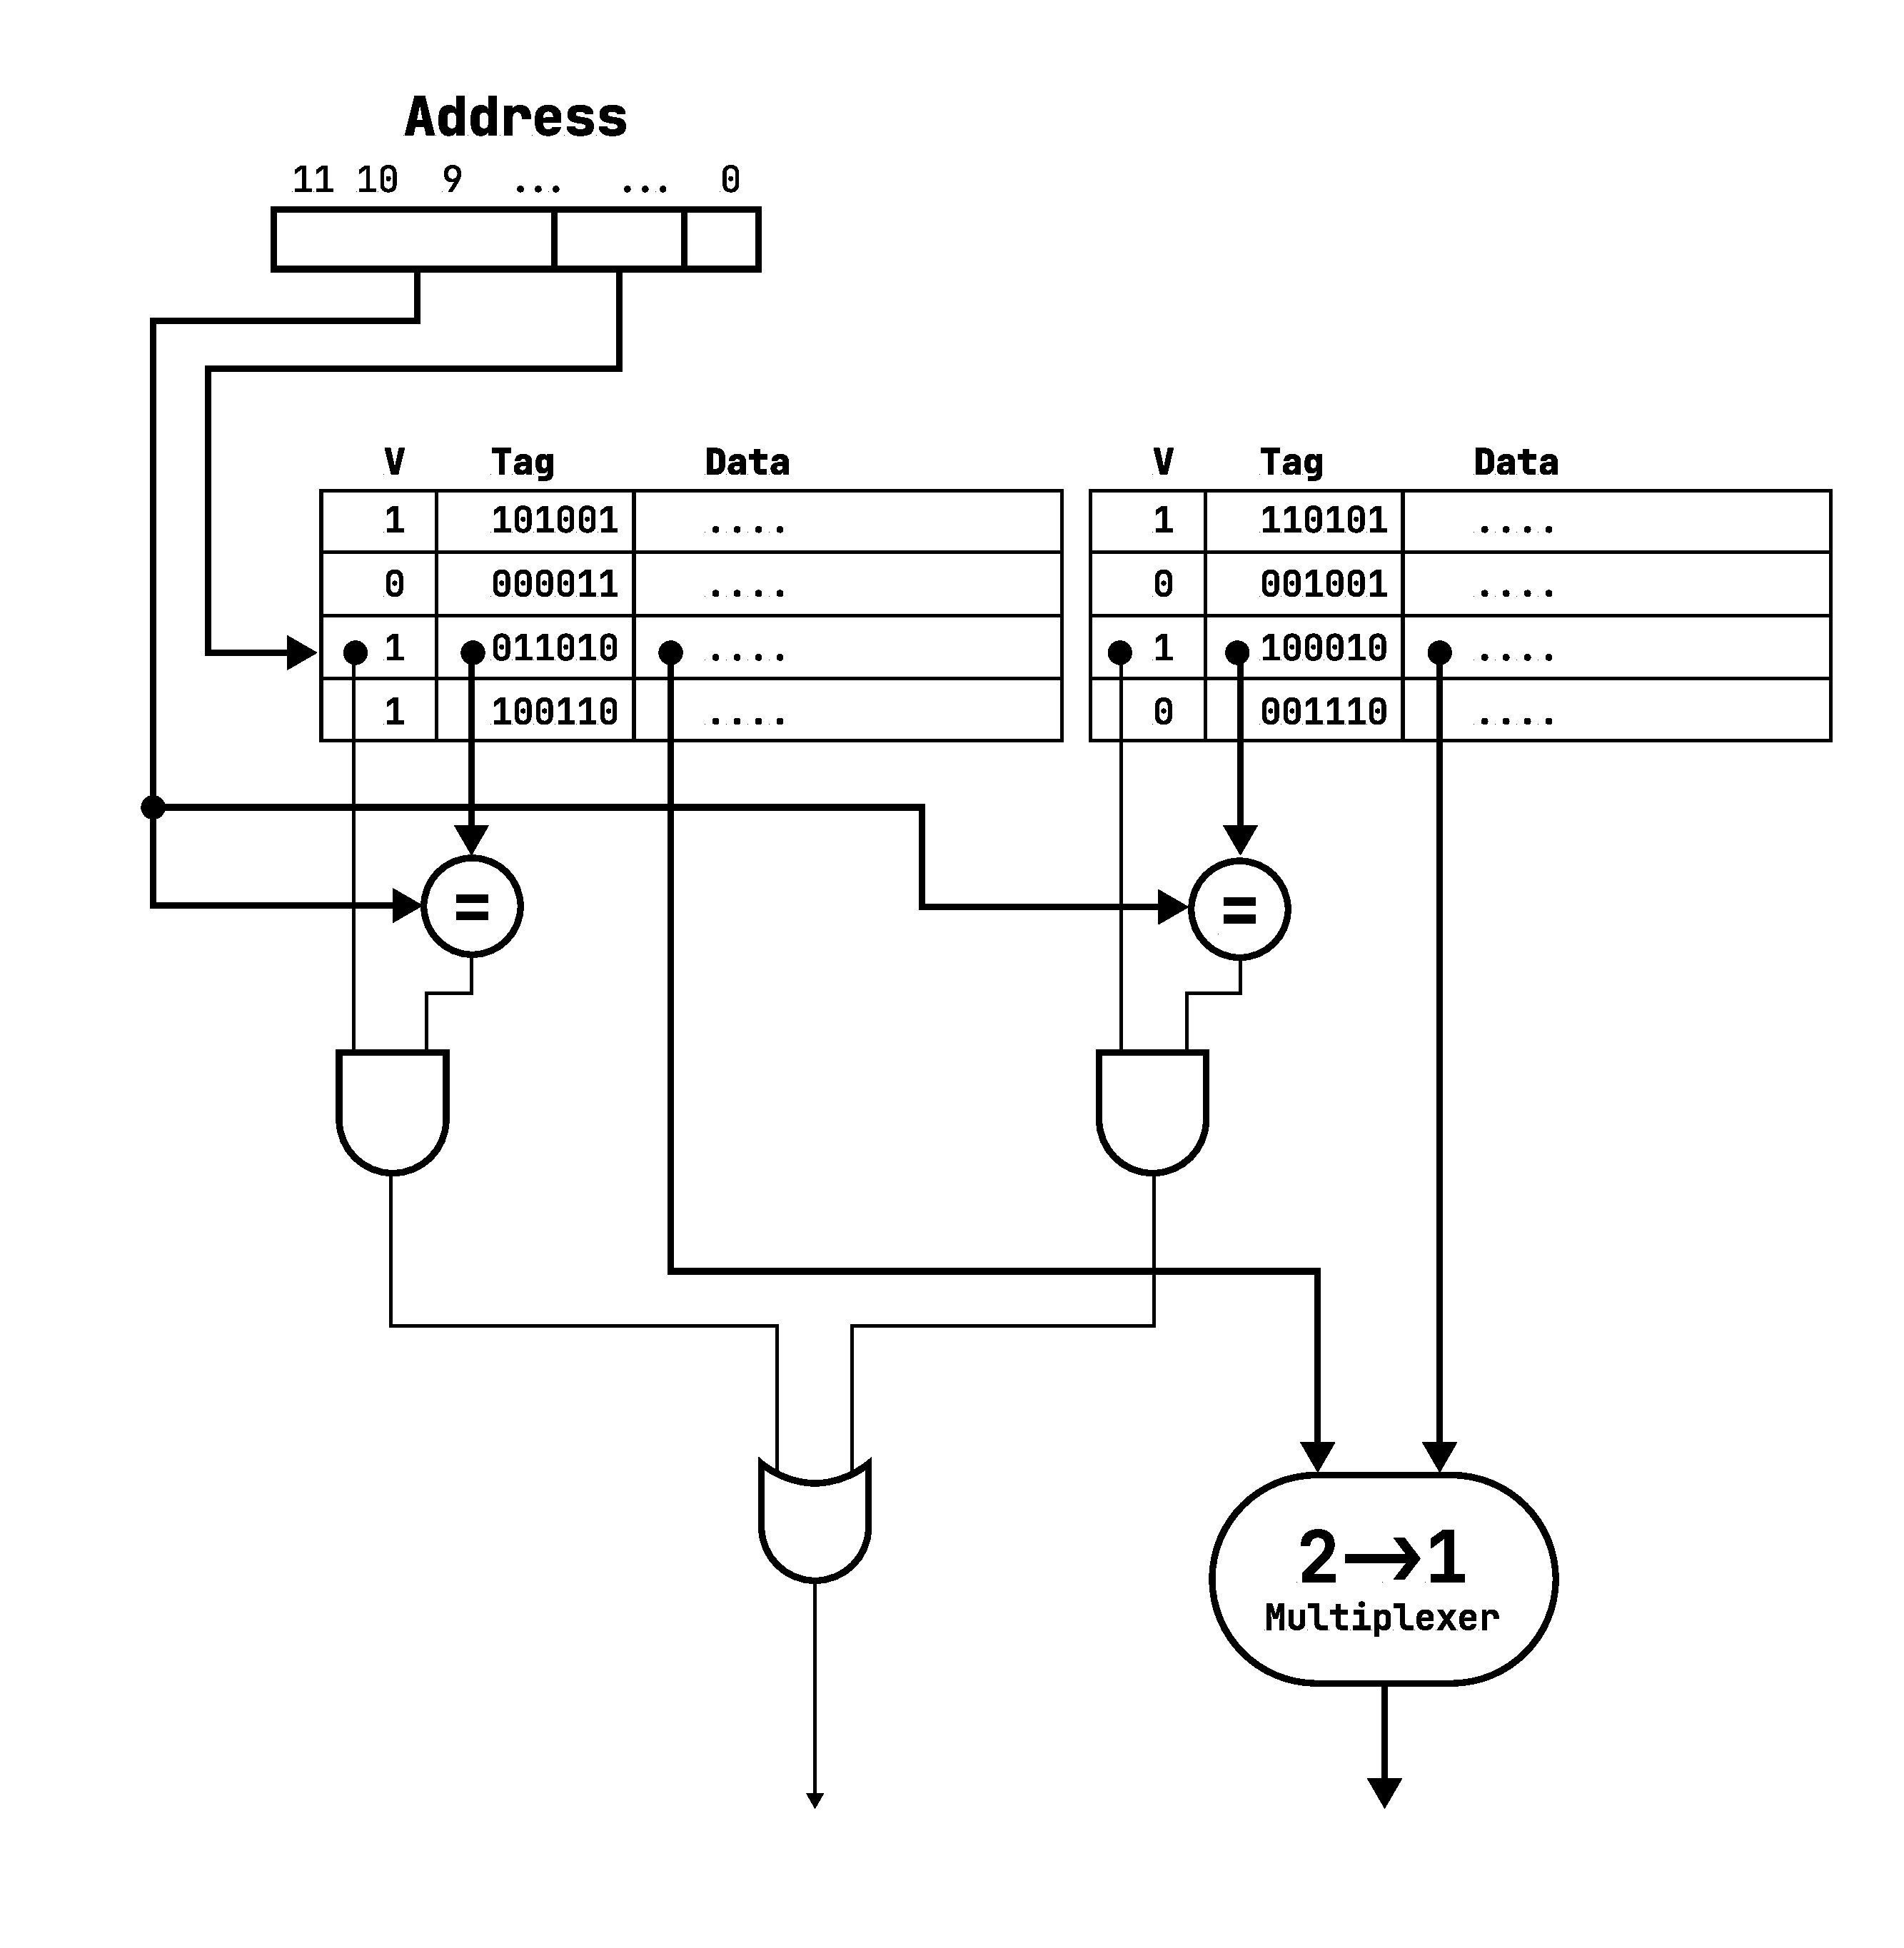
\includegraphics[width=0.9\textwidth]{img/layout.pdf}
    \caption{Layout for a cache implementation}
    \label{fig:layout}
\end{figure}

\newpage

\begin{questions}

\question[2] In Figure \ref{fig:layout}, what is a row stands for?
{

    \begin{oneparchoices}
        \choice One set.
        \choice One cache block.
        \choice One entire cache.
        \choice Not listed in choices.
    \end{oneparchoices}
    
    \begin{solution}
        \begin{oneparcheckboxes}
            %%%%%%%%%%% YOUR ANSWER HERE %%%%%%%%%%%%%%%%%%%%%%%%%%%%
            % If you find the correct answer, substitute `\choice` by
            % `\CorrectChoice`!
            %%%%%%%%%%%%%%%%%%%%%%%%%%%%%%%%%%%%%%%%%%%%%%%%%%%%%%%%%
            \CorrectChoice A
            \choice B
            \choice C
            \choice D
        \end{oneparcheckboxes}
    \end{solution}

}

\question[2] In Figure \ref{fig:layout}, what is \texttt{V} stands
for?
{

    \begin{oneparchoices}
        \choice Valid bit.
        \choice Vacant bit.
        \choice Visited bit.
    \end{oneparchoices}
    
    \begin{solution}
        \begin{oneparcheckboxes}
            %%%%%%%%%%% YOUR ANSWER HERE %%%%%%%%%%%%%%%%%%%%%%%%%%%%
            % If you find the correct answer, substitute `\choice` by
            % `\CorrectChoice`!
            %%%%%%%%%%%%%%%%%%%%%%%%%%%%%%%%%%%%%%%%%%%%%%%%%%%%%%%%%
            \CorrectChoice A
            \choice B
            \choice C
        \end{oneparcheckboxes}
    \end{solution}

}

\question[2] What is the type of the cache described in Figure \ref{fig:layout}?
{

    \begin{choices}
        \choice Direct-Mapped cache.
        \choice Set-Associative Cache (If you choose this, write
        down its associativity).
        \choice Fully-Associative Cache (If you choose this, write
        down its associativity).
    \end{choices}
    
    \begin{solution}
        \begin{checkboxes}
            %%%%%%%%%%% YOUR ANSWER HERE %%%%%%%%%%%%%%%%%%%%%%%%%%%%
            % If you find the correct answer, substitute `\choice` by
            % `\CorrectChoice`!
            % If you choose B or C, write your answer in `\fillin[]`
            % arguments.
            %%%%%%%%%%%%%%%%%%%%%%%%%%%%%%%%%%%%%%%%%%%%%%%%%%%%%%%%%
            \choice A
            % Write your answer in `\fillin[]` arguments!
            \CorrectChoice B (Associativity: \fillin[2])
            % Write your answer in `\fillin[]` arguments!
            \choice C (Associativity: \fillin[])
        \end{checkboxes}
    \end{solution}

}

\question[3] What is the ( Tag : Set Index : Byte Offset ) breakdown
of memory addresses in Figure \ref{fig:layout}?
{
    \begin{solution}
        \begin{enumerate}
            %%%%%%%%%%% YOUR ANSWER HERE %%%%%%%%%%%%%%%%%%%%%%%%%%%%
            % Write your answer in `\fillin[]` arguments!
            %%%%%%%%%%%%%%%%%%%%%%%%%%%%%%%%%%%%%%%%%%%%%%%%%%%%%%%%%
            \item Tag:         \fillin[11:6]
            \item Index:       \fillin[5:4]
            \item Byte Offset: \fillin[3:0]
        \end{enumerate}
    \end{solution}

}

\question[2] Is it TRUE that conflict misses cannot occur in
fully-associated caches?
{

    \begin{oneparchoices}
        \choice Yes.
        \choice No.
    \end{oneparchoices}
    
    \begin{solution}
        \begin{oneparcheckboxes}
            %%%%%%%%%%% YOUR ANSWER HERE %%%%%%%%%%%%%%%%%%%%%%%%%%%%
            % If you find the correct answer, substitute `\choice` by
            % `\CorrectChoice`!
            %%%%%%%%%%%%%%%%%%%%%%%%%%%%%%%%%%%%%%%%%%%%%%%%%%%%%%%%%
            \CorrectChoice A
            \choice B
        \end{oneparcheckboxes}
    \end{solution}

}

\newpage

\question[3] Tell the difference(s) between Conflict Miss and
Capacity Miss.
{

    \begin{solution}
            %%%%%%%%%%% YOUR ANSWER HERE %%%%%%%%%%%%%%%%%%%%%%%%%%%%
            
            % \begin{enumerate}
            %     \item 
            % \end{enumerate}
            
            \textbf{Conflict Miss} is caused because of multiple memory locations mapped to the same location of cache, while \textbf{Capacity Miss} is because of the cache is not big enough to contain all blocks accessed by the program.

            If a cache miss occurs (this address has been refrenced before, meaning it cannot be compulsory miss), then we can go through the entire string of accesses with a fully associative cache with an LRU replacement policy. In this scenario, if a cache hit occurs, then it indicates \textbf{Conflict Miss}. Otherwise if a cache miss happens, then it indicates \textbf{Capacity Miss}.

            % Suppose that we went through the entire string of accesses with a fully associative cache (with LRU replacement policy), and the initial address hits, then it is called 'conflict miss'. Otherwise (if the initial address miss), it is a capacity miss.
            % \vspace{1in}
            %%%%%%%%%%%%%%%%%%%%%%%%%%%%%%%%%%%%%%%%%%%%%%%%%%%%%%%%%
    \end{solution}

}


\question[12] For each of the following accesses to the cache
described in Figure \ref{fig:layout}, determine if each
access would be a hit or miss based on the cache state shown above.
If it is a miss, classify the miss type(s). \label{access_simulate}

If multiple miss types may exist depending on prior memory accesses,
select \emph{all possible} miss types. For each access, you will get
\begin{itemize}
    \item 2 points if you choose all correct choice(s),
    \item 1 point if you choose partial correct choice(s), and,
    \item 0 point if you give no choice(s) or wrong choice(s).
\end{itemize}

Each memory access should be considered \emph{dependently}.
In particular, \emph{Do update} the cache status after each memory
access. If a replacement happens, data in the first slot will 
always be evicted.

% Hint: Consider the cache as Fully-Associative before judging whether
% a miss is capacity miss.

\begin{table}[h]
    \centering
    \begin{tabular}{l l l}
        \hline % -------------------------------------------------
        Order & Address                   & Access Outcome \\
        \hline % -------------------------------------------------
        1     & \texttt{0b 101001 000100} & \fillin[1]\\
        2     & \texttt{0b 011010 110100} & \fillin[2]\\
        3     & \texttt{0b 111110 101000} & \fillin[3]\\
        4     & \texttt{0b 000011 111100} & \fillin[4]\\
        5     & \texttt{0b 000011 011001} & \fillin[5]\\
        6     & \texttt{0b 100110 101100} & \fillin[6]\\
        \hline % -------------------------------------------------
    \end{tabular}
\end{table}

{

    \begin{solution}\\
        Note: Each access may have one or more correct choice(s).
        \begin{enumerate}
            \item 
            {
                %%%%%%%%%%% 1. YOUR ANSWER HERE %%%%%%%%%%%%%%%%%%
                % If you find the correct answer, substitute 
                % `\choice` by `CorrectChoice`!
                %%%%%%%%%%%%%%%%%%%%%%%%%%%%%%%%%%%%%%%%%%%%%%%%%%
                \begin{oneparcheckboxes}
                    \CorrectChoice Hit
                    \choice Compulsory Miss
                    \choice Conflict Miss
                \end{oneparcheckboxes}
            }
            \item 
            {
                %%%%%%%%%%% 2. YOUR ANSWER HERE %%%%%%%%%%%%%%%%%%
                % If you find the correct answer, substitute 
                % `\choice` by `CorrectChoice`!
                %%%%%%%%%%%%%%%%%%%%%%%%%%%%%%%%%%%%%%%%%%%%%%%%%%
                \begin{oneparcheckboxes}
                    \choice Hit
                    \CorrectChoice Compulsory Miss
                    \CorrectChoice Conflict Miss
                \end{oneparcheckboxes}
            }
            \item 
            {
                %%%%%%%%%%% 3. YOUR ANSWER HERE %%%%%%%%%%%%%%%%%%
                % If you find the correct answer, substitute 
                % `\choice` by `CorrectChoice`!
                %%%%%%%%%%%%%%%%%%%%%%%%%%%%%%%%%%%%%%%%%%%%%%%%%%
                \begin{oneparcheckboxes}
                    \choice Hit
                    \CorrectChoice Compulsory Miss
                    \CorrectChoice Conflict Miss
                \end{oneparcheckboxes}
            }
            \item 
            {
                %%%%%%%%%%% 4. YOUR ANSWER HERE %%%%%%%%%%%%%%%%%%
                % If you find the correct answer, substitute 
                % `\choice` by `CorrectChoice`!
                %%%%%%%%%%%%%%%%%%%%%%%%%%%%%%%%%%%%%%%%%%%%%%%%%%
                \begin{oneparcheckboxes}
                    \choice Hit
                    \CorrectChoice Compulsory Miss
                    \CorrectChoice Conflict Miss
                \end{oneparcheckboxes}
            }
            \item 
            {
                %%%%%%%%%%% 5. YOUR ANSWER HERE %%%%%%%%%%%%%%%%%%
                % If you find the correct answer, substitute 
                % `\choice` by `CorrectChoice`!
                %%%%%%%%%%%%%%%%%%%%%%%%%%%%%%%%%%%%%%%%%%%%%%%%%%
                \begin{oneparcheckboxes}
                    \choice Hit
                    \CorrectChoice Compulsory Miss
                    \choice Conflict Miss
                \end{oneparcheckboxes}
            }
            \item 
            {
                %%%%%%%%%%% 6. YOUR ANSWER HERE %%%%%%%%%%%%%%%%%%
                % If you find the correct answer, substitute 
                % `\choice` by `CorrectChoice`!
                %%%%%%%%%%%%%%%%%%%%%%%%%%%%%%%%%%%%%%%%%%%%%%%%%%
                \begin{oneparcheckboxes}
                    \choice Hit
                    \CorrectChoice Compulsory Miss
                    \CorrectChoice Conflict Miss
                \end{oneparcheckboxes}
            }
        \end{enumerate}
    \end{solution}

}

\newpage

\question[6] 
The specification sheet of the system is given below. What is the
Average Memory Access Time (AMAT) of memory accesses in
Question \ref{access_simulate}?
What is the AMAT if we remove this cache? Please give your answer
in nanosecond (ns). You shall have the formula, the unit of
results and the deriving procedure presented in your answer.
(Note: A 1 gigahertz (GHz) processor ticks a cycle for each 1
nanosecond)

\begin{table}[h]
    \centering
    \begin{tabular}{l l}
        \hline % ---------------------------------
        System Frequency           & 2 GHz      \\
        Cache Access Latency       & 2 Cycles   \\
        Main Memory Access Latency & 600 Cycles \\
        \hline % ---------------------------------
    \end{tabular}
    \caption{Specification Sheet}
    \label{tab:spec_sheet}
\end{table}

{
    \begin{solution}
        %%%%%%%%%%%%%% YOUR ANSWER HERE %%%%%%%%%%%%%%%%%%%%%%%%%

        \begin{enumerate}
            \item Time for one clock cycle = 1 / System frequency = 0.5ns

            Hit time = Cache Access Latency = 2 Cycles = 1ns
    
            Miss Penalty = Main Memory Access Latency = 600 Cycles = 300ns
    
            AMAT = hit time + miss rate $\times$ miss penalty
    
            \ \ \ \ \ \ \ \ \ \ = 1 + $\frac{5}{6}$ $\times$ 300
    
            \ \ \ \ \ \ \ \ \ \ = 251ns

            \item If we remove the cache, the access time will always be 600 cycles, and the AMAT will be 

            AMAT = (600 cycles) $\times$ 0.5 ns = 300ns
        \end{enumerate}

        %%%%%%%%%%%%%%%%%%%%%%%%%%%%%%%%%%%%%%%%%%%%%%%%%%%%%%%%%
        \vspace{2in}
    \end{solution}
}

\end{questions}
\newpage
% From TA: Please go to `overbyte.tex` to typeset your answers for
% section 2! Your answer will be reflected.
%%%%%%%%%%%%%%%%%%%%%%%%%%%%%%%%%%%%%%%%%%%%%%%%%%%%%%%%%%%%%%%%%%%%%
% This is a LaTeX template for students
% working on Homework 6, Computer Architecture I, Spring, 2022.
% You SHALL NOT distribute this template.
%%%%%%%%%%%%%%%%%%%%%%%%%%%%%%%%%%%%%%%%%%%%%%%%%%%%%%%%%%%%%%%%%%%%%
\section{Oops \dots Too many bites (bytes)}
In this sections, we will review the implementation of caches and
replacement policies.

\begin{questions}

\question[15] Let's Draw It Out!

Sketch the organization of a \emph{four-way set associative} cache
with a cache block size of 16 bytes and a total size of 128 bytes.
Your sketch should have a style similar to Figure 1. The memory
addresses are 12-bit long.

In your sketch, the following components should be also presented.

\begin{enumerate}
    \item the width of set index, tag and data fields of memory
    addresses (3 points),
    \item logical components used for comparison and selection
    (2 points),
    \item the type of multiplexer (e.g. $2\rightarrow1$,
    $4\rightarrow1$, $8\rightarrow1$, $16\rightarrow1$, etc.)
    (1 point),
    \item the number of sets (1 point) , and,
    \item an implementation layout including wiring and placement
    of cache elements (8 points).
\end{enumerate}



{
    \begin{solution}
    % DRAWING BY HAND IS HIGHLY RECOMMENDED!
    % You are not recommended to draw it with LaTeX, as it will
    % take you TREMENDOUS time. Let's make our life more easier :)
    % So, please attach your figures in `img/` directory and use
    % \includegraphics{}
    % to display it here.

    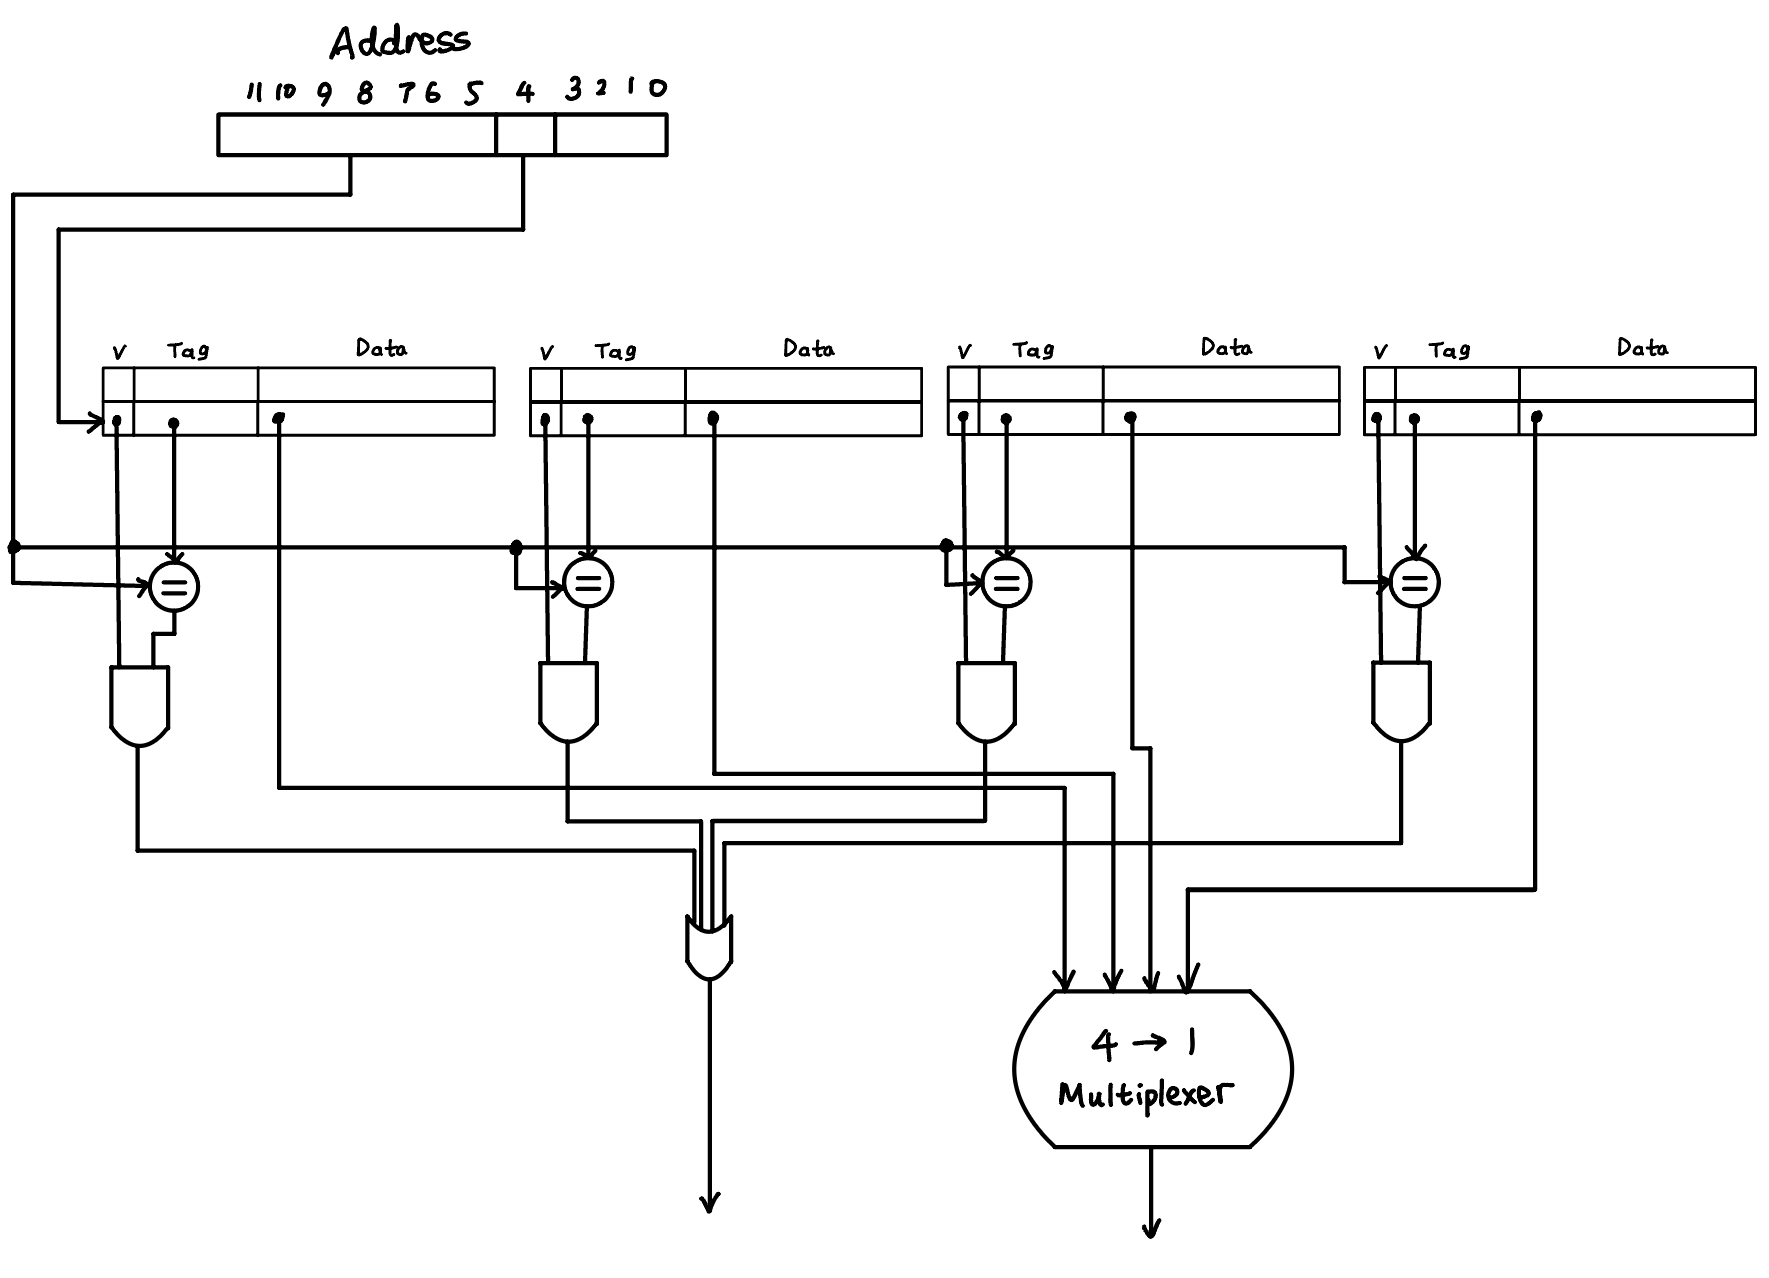
\includegraphics[scale=0.25]{q2.jpeg}

    \vspace{5in}
    \end{solution}
}
\newpage

In the following questions, we will examine how replacement policies
affect miss rate.

After the system is cold start, the address sequence of warm-up
accesses is:\\
\texttt{0x2A, 0x3C, 0x7D, 0xCE, 0x5B, 0x01, 0x2C, 0x1D, 0x9B, 0x3E}.

After all warm-up accesses are done, the address sequence of
follow-up accesses is: \\
\texttt{0x30, 0x40, 0x52, 0x44, 0x56, 0x48, 0x5A, 0x4C, 0x10, 0x3B,
0x5C, 0x30, 0x5E}.

\question[2] Which locality(s) can you observe in the follow-up
accesses?

{

    \begin{solution}
        Note: There may exist(s) one or more correct choice(s).\\
        \begin{oneparcheckboxes}
            \CorrectChoice Spatial locality
            \CorrectChoice Temporal locality
        \end{oneparcheckboxes}
    \end{solution}

}

\question[2] Assume \emph{Least Recently Used} (LRU) replacement
policy is applied. Circle out all access(es) with cache hit in
the follow-up accesses. \label{q:lru}

{
    \begin{solution}
        % Use \Circled{} to surround the access you want to choose.
        Circle the access(es) that meets a cache hit!
        (like this: \texttt{\Circled{0xFF}})\\
        \begin{center}
        \texttt{\Circled{0x30}, 0x40, \Circled{0x52}, \Circled{0x44}, \Circled{0x56}, \Circled{0x48}, \Circled{0x5A}, \Circled{0x4C}, \Circled{0x10},
        \Circled{0x3B}, \Circled{0x5C}, \Circled{0x30}, \Circled{0x5E}}.
        \end{center}
        \vspace{7px}
    \end{solution}
}

\question[2] Assume \emph{Most Recently Used} (MRU) replacement policy
is applied. Circle out all access(es) with cache hit in the follow-up
accesses. \label{q:mru}

{
    \begin{solution}
        % Use \Circled{} to surround the access you want to choose.
        Circle the access(es) that meets a cache hit!
        (like this: \texttt{\Circled{0xFF}})\\
        \begin{center}
        \texttt{\Circled{0x30}, 0x40, \Circled{0x52}, \Circled{0x44}, \Circled{0x56}, \Circled{0x48}, \Circled{0x5A}, \Circled{0x4C}, 0x10,
        \Circled{0x3B}, 0x5C, 0x30, 0x5E}.
        \end{center}
        \vspace{7px}
    \end{solution}
}

\question[6] 
The specification sheet of the system is given below. What is the
Average Memory Access Time (AMAT) of memory accesses in the question
\ref{q:lru} and \ref{q:mru}? Please give your answer in nanosecond 
(ns). You shall have the formula, the unit of results and the
deriving procedure presented in your answer. (Note: A 1 gigahertz
(GHz) processor ticks a cycle for each 1 nanosecond)

\begin{table}[h]
    \centering
    \begin{tabular}{l l}
        \hline % ---------------------------------
        System Frequency           & 2 GHz      \\
        Cache Access Latency       & 2 Cycles   \\
        Main Memory Access Latency & 130 Cycles \\
        \hline % ---------------------------------
    \end{tabular}
    \caption{Specification Sheet}
    \label{tab:spec_sheet}
\end{table}

{
    \pagebreak
    \begin{solution}
        %%%%%%%%%%%%%% YOUR ANSWER HERE %%%%%%%%%%%%%%%%%%%%%%%%%

        In both problems, 

        Time for one clock cycle = 1 / System frequency = 0.5ns

        Hit time = Cache Access Latency = 2 Cycles = 1ns

        Miss Penalty = Main Memory Access Latency = 130 Cycles = 65ns

        \begin{enumerate}
            \item In problem 3, the Miss Rate is $1/13$
            
            AMAT = hit time + miss rate $\times$ miss penalty

            \ \ \ \ \ \ \ \ \ \ = 1 + $\frac{1}{13} \times $ 65

            \ \ \ \ \ \ \ \ \ \ = 6ns

            \item In problem 4, the Miss Rate is $5/13$
            
            AMAT = hit time + miss rate $\times$ miss penalty

            \ \ \ \ \ \ \ \ \ \ = 1 + $\frac{5}{13} \times $ 65

            \ \ \ \ \ \ \ \ \ \ = 26ns

        \end{enumerate}

        %%%%%%%%%%%%%%%%%%%%%%%%%%%%%%%%%%%%%%%%%%%%%%%%%%%%%%%%%
        \vspace{1in}
    \end{solution}
}


\end{questions}

\newpage
% From TA: Please go to `practical.tex` to typeset your answers for
% section 3! Your answer will be reflected.
%%%%%%%%%%%%%%%%%%%%%%%%%%%%%%%%%%%%%%%%%%%%%%%%%%%%%%%%%%%%%%%%%%%%%
% This is a LaTeX template for students
% working on Homework 6, Computer Architecture I, Spring, 2022.
% You SHALL NOT distribute this template.
%%%%%%%%%%%%%%%%%%%%%%%%%%%%%%%%%%%%%%%%%%%%%%%%%%%%%%%%%%%%%%%%%%%%%
\section{Let's See Some Real World Example}

Each time when you access the course website, your activity will be
recorded into our web server logs! This is the definition of the web
server log for our Computer Architecture course website. Assume our
web server is a 32-bit machine. In this question, we will examine
code optimizations to improve log processing speed. The data
structure for the log is defined below.
\begin{minted}{c}
    struct log_entry {
        int src_ip;    /* Remote IP address */
        char URL[128]; /* Request URL. You can consider 128 characters are enough. */
        long reference_time; /* The time user referenced to our website. */
        char browser[64]; /* Client browser name */
        int status; /* HTTP response status code. (e.g. 404) */
    } log[NUM_ENTRIES];
\end{minted}
Assume the following processing function for the log. This function
determines the most frequently observed source IPs during the given
hour that succeed to connect our website.

\begin{minted}{c}
    topK_success_sourceIP (int hour);
\end{minted}

\begin{questions}

\question[2] Which field(s) in a log entry will be accessed for the
given log processing function?

{
    \begin{solution}
        Note: There may exist(s) one or more correct choice(s).\\
        % If you find the correct answer, substitute `\choice`
        % by `CorrectChoice`!
        \begin{oneparcheckboxes}
            \CorrectChoice \texttt{src\_ip}
            \choice \texttt{URL}
            \CorrectChoice \texttt{reference\_time}
            \choice \texttt{browser}
            \CorrectChoice \texttt{status}
        \end{oneparcheckboxes}
    \end{solution}
}

\question[1] Assuming 32-byte cache blocks and no prefetching, how
many cache misses per entry does the given function incur on average? \label{q:miss}

{
    \begin{solution}
        % fill your answer in \fillin arguments.
        \fillin[2.25][4in]
    \end{solution}
}

\question[3] How can you reorder the data structure to improve
cache utilization and access locality? Justify your modification.

{
    \begin{solution}

        \textbf{Reordered data structure:}

        We can improve cache utilization by reordering the struct members, putting the three needed values together. Considering memory alignment, we use a struct with \texttt{int, int, long} rather than \texttt{int, long, int}.
        \begin{minted}{c}
struct log_entry {
    int src_ip;   
    int status; 
    long reference_time; 
    char URL[128]; 
    char browser[64];
} log[NUM_ENTRIES];
        \end{minted}

        \textbf{Justification:}

        In this case, after the first time we visit `\texttt{int src\_ip}' and get a compulsory miss, both `\texttt{long reference\_time}' and `\texttt{int status}' can be loaded in our 32-byte cache. Therefore the next two accesses to them will be cache hits, thanks to spacial locality. Now the cache is filled with `\texttt{int src\_ip, int status, long reference\_time}' and the beginning 16-bytes of \texttt{char URL[128]}. 

        When accessing the 2nd log entry, the cache will be filled with the last 32 bytes of \texttt{char browser[64]} along with the \texttt{int src\_ip, int status, long reference\_time} of the second struct. 

        When accessing the 3rd log entry, the cache status is the same as the 1st log entry. Therefore accessing every two structs yields 2 cache misses, thus on average, only 1 cache miss will occur on each entry.
        
        \textbf{Cache misses per entry:}
        
        On average, 1 cache miss per entry.
        
        % Compared to the original data structure, only 1 cache miss will occur on each entry.

    \end{solution}
}

\newpage

\question[6] To mitigate the miss in the question \ref{q:miss},
design a different data structure. How would you rewrite the
program to improve the overall performance?

Your answer shall include:

\begin{itemize}
    \item A new layout of data structure of our server logs.
    \item A description of how your function would improve the
    overall performance.
    \item How many cache misses per entries does your improved
    design incur on average?
\end{itemize}

{
    \begin{solution}
        %%%%%%%%%%%%%% YOUR ANSWER HERE %%%%%%%%%%%%%%%%%%%%%%%%%
        
        \textbf{New layout of design}:

        We can separate the struct into two structs. % Additionally, put the int together (int, int, long, instead of int, long, int), which minimizes the struct considering memory alignment.

        \begin{minted}{c}
    struct log_entry_1 {
        int src_ip;  
        int status; 
        long reference_time;
    } log_1[NUM_ENTRIES];

    struct log_entry_2 {
        char URL[128]; 
        char browser[64]; 
    } log_2[NUM_ENTRIES];

        \end{minted}

        \textbf{Description}:

        If we separate the accessed variables and unused variables apart, the function only needs to check the values in the first struct, namely `\texttt{struct log\_entry\_1}'. Additionally, put the int together (int, int, long, instead of int, long, int), which minimizes the struct considering memory alignment.

        Since the size of this struct is 16 bytes, and they are placed continously in memory, we can store two structs in one 32-byte cache block. Therefore, after the first cache miss, the next 5 references (the remaining accesses of the two adjacent entries) will all become cache hits. This can significantly improve the overall performance.\newline

        \textbf{Cache misses per entry}:

        Since there're only 1 cache miss out of two entries, the average cache misses per entry is $0.5$.

        % In the new design, the function only needs to check the values in the first struct. Since the accessed things are placed together in memory (instead of separated by the quite big `URL' and `browser' data), we can take advantage of the spacial locality. Visits to the second entry can benefit from the previous entry, eliminating cache misses further.

        % The size of the first struct (struct log\_entry\_1) is 16 bytes, and our cache line is 32 bytes. Two entries can be placed in one cache line. Therefore the average cache misses per entries is $0.5$.

        %%%%%%%%%%%%%%%%%%%%%%%%%%%%%%%%%%%%%%%%%%%%%%%%%%%%%%%%%
        \vspace{4in}
    \end{solution}
}

\end{questions}
%% THINGS BELOW SHOULD BE LEFT UNTOUCHED %%%%%%%%%%%%%%%%%%%%%%%%%%%%
%%%%%%%%%%%%%%%%%%%%%%%%%%%%%%%%%%%%%%%%%%%%%%%%%%%%%%%%%%%%%%%%%%%%%
% This is a LaTeX template for students
% working on Homework 6, Computer Architecture I, Spring, 2022.
% You SHALL NOT distribute this template.
%%%%%%%%%%%%%%%%%%%%%%%%%%%%%%%%%%%%%%%%%%%%%%%%%%%%%%%%%%%%%%%%%%%%%
\section*{One more thing...}
Phew! That's all about cache! Tell us your feeling after finish this
homework. Thank You! Don't worry if you did not assign this to
Gradescope. This part is \emph{optional}.

\begin{questions}

\question[0] How do you \emph{feel} after you have done this homework?

{
    \begin{solution}
        \begin{checkboxes}
            \CorrectChoice :) I feel good.
            \choice :( I feel bad.
        \end{checkboxes}
    \end{solution}
}

\question[0] Do you think this homework is hard for you?

{
    \begin{solution}
        \begin{checkboxes}
            \choice It's really difficult for me!
            \choice I think it is a little bit challenging.
            \CorrectChoice I am okay with that.
            \choice This is too easy for me.
        \end{checkboxes}
    \end{solution}
}

\question[0] Your voice will be secretly heard by our team.
Is there anything you want to feedback?

{
    \begin{solution}
        \vspace{1in}
    \end{solution}
}

\vspace*{\fill}
\begin{center}
\Large Thank you! Now you are clear with cache! :)
\end{center}

\end{questions}

\end{document}
